\section{Additional Results}
\label{app:grids}

Cells are means $\pm$ sample standard deviation over the stated number of seeds. A seed that
finishes above 95\,\% of the unigram perplexity counts as collapsed and is not averaged
(except in \Cref{tab:fullrank}):
\textit{n/m collapsed} means $n$ of $m$ seeds collapsed. An italic range replaces the mean when
no seed collapsed but the seeds disagree (largest at least $1.5\times$ the smallest, or a
standard deviation above 15\,\% of the mean).

\subsection{Reproducibility}
\label{app:res-repro}

The undamped configuration at the original temperature ($\nlab=16$, $6{,}000$ steps) ends at
$430.0$ on an NVIDIA A40 and at $645.0$ on a TITAN~RTX (\Cref{sec:exp-repro}). A rerun on an A40
reproduces the whole twelve-point validation trace to every printed digit; the TITAN~RTX trace
begins $711.6$, $640.3$, $686.0$. The first evaluations already differ ($711.70$
against $711.61$), so the runs diverge within $500$ steps; the gap then grows to $215$ perplexity. Nothing
differs but the order of floating-point reductions: on one device, two versions of the
implementation and two training drivers, in three combinations, agree to every printed digit.

Seeds act the same way. Three seeds on one device give $610.9$, $408.8$ and $367.5$
($\ReproUndampedMean\pm\ReproUndampedSd$). The same \ReproDampedN{} seeds damped with
$\alpha_Z=0.25$ give $\ReproDampedMean\pm\ReproDampedSd$, a standard deviation of
\ReproDampedPct\,\% of the mean, \ReproSdRatio{} times tighter (\Cref{fig:repro}). In this
regime single-seed comparisons are not informative. A global variable moves an undamped model at $\nlab=24$ from $321.4$ to $297.7$
with one seed each, a difference of $23.7$ against a seed standard deviation of
$\ReproUndampedSd$. A single-seed comparison of damping gives $641.5$ against $248.3$; damping
improves reproducibility at least as much as the mean. The damped configuration at $\nlab=32$ is reproducible: $253.0\pm6.0$ over three
seeds, against $250.7\pm2.3$ from an independent set of runs.

\begin{figure}[t]
\centering
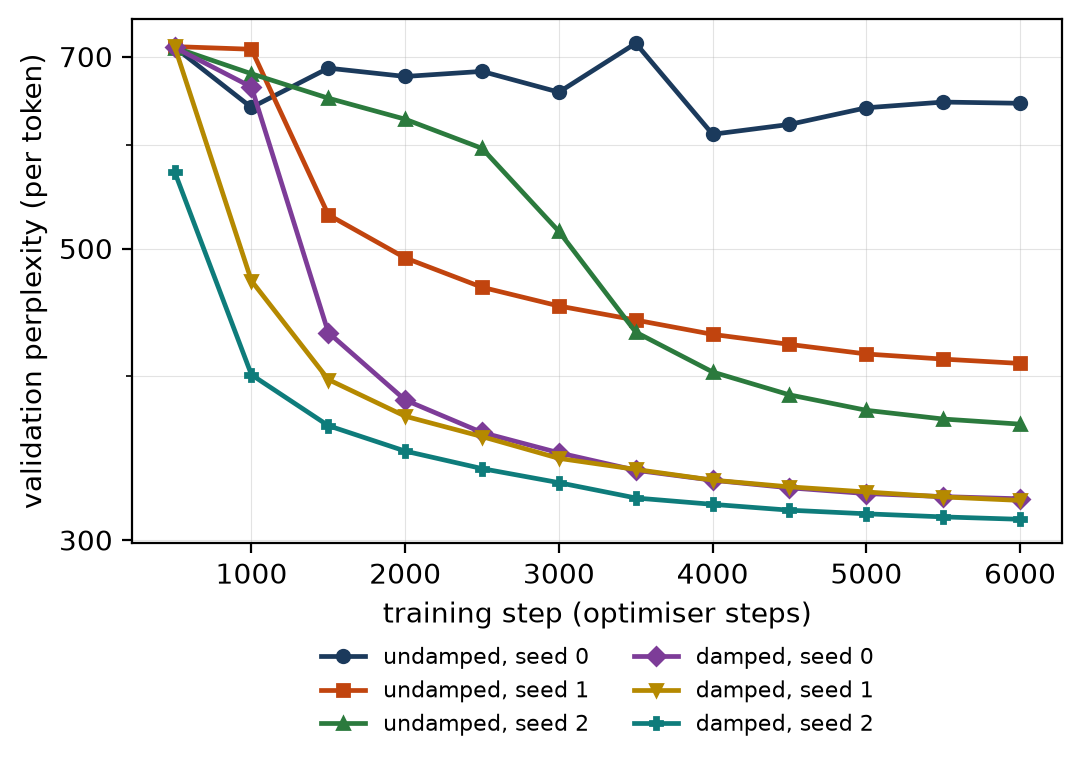
\includegraphics[width=0.85\columnwidth]{figures/fig_repro_seeds.png}
\caption{One undamped configuration at the original temperature, three seeds each without and
with damping ($\alpha_Z=0.25$). Undamped runs separate by more than $200$ perplexity and do not
reconverge; damped runs are indistinguishable after $3{,}000$ steps. Curves are validation
traces; the text quotes best-validation checkpoints, so a curve may end above its quoted value.}
\label{fig:repro}
\end{figure}

\subsection{Scaling}
\label{app:grid-exponents}

The transformer gives $129.2$ at $\dmodel=64$, $124.7$ at $160$ and $125.3$ at $256$, while its
training perplexity falls from $68.5$ to $10.2$: on $929{,}589$ training tokens it is limited by
data. At matched non-embedding budget the looped transformer is better at small sizes ($164.7$ at
$12{,}768$ parameters against $195.2$ at $13{,}152$) and worse at large ones ($135.7$ at
$198{,}528$ against $129.2$ at $200{,}064$). At matched total parameters the standard
transformer wins everywhere (\Cref{fig:scaling-total}).

A model's frontier is its best-of-two-learning-rates point at each size. Fitted over each
curve's own range, the exponents are $\OwnTf$ (transformer), $\OwnLp$ (looped),
$\OwnPt$ (full-rank causal PT, standardised temperature) and $\OwnLow$ (low-rank causal PT). The
first three look alike only because the baselines extend to $1.2\times10^6$ parameters, where
flat points pull their slopes down; from the same runs, the looped transformer gives
$\ExpTfvLpLp$ over the transformer's range and $\ExpLpvPtLp$ over the causal PT's. The full-rank
causal PT is absent from \Cref{tab:exponents-trio} because the looped frontier has only two
points on the range it shares with both baselines. In the pairwise fits of
\Cref{tab:exponents-full} the ordering is the same in all five pairs, and the leave-one-out
ranges are disjoint in every pair with enough points to compute them.

Causal PT entries are seed means, and the best seed can differ from the mean by more than the
effects we discuss: at $\nlab=\SpreadLab$, $\krank=\SpreadRank$ the best of \SpreadSeeds{} seeds
gives $\SpreadBest$ and the mean is $\SpreadMean\pm\SpreadSd$.

\begin{figure}[t]
\centering
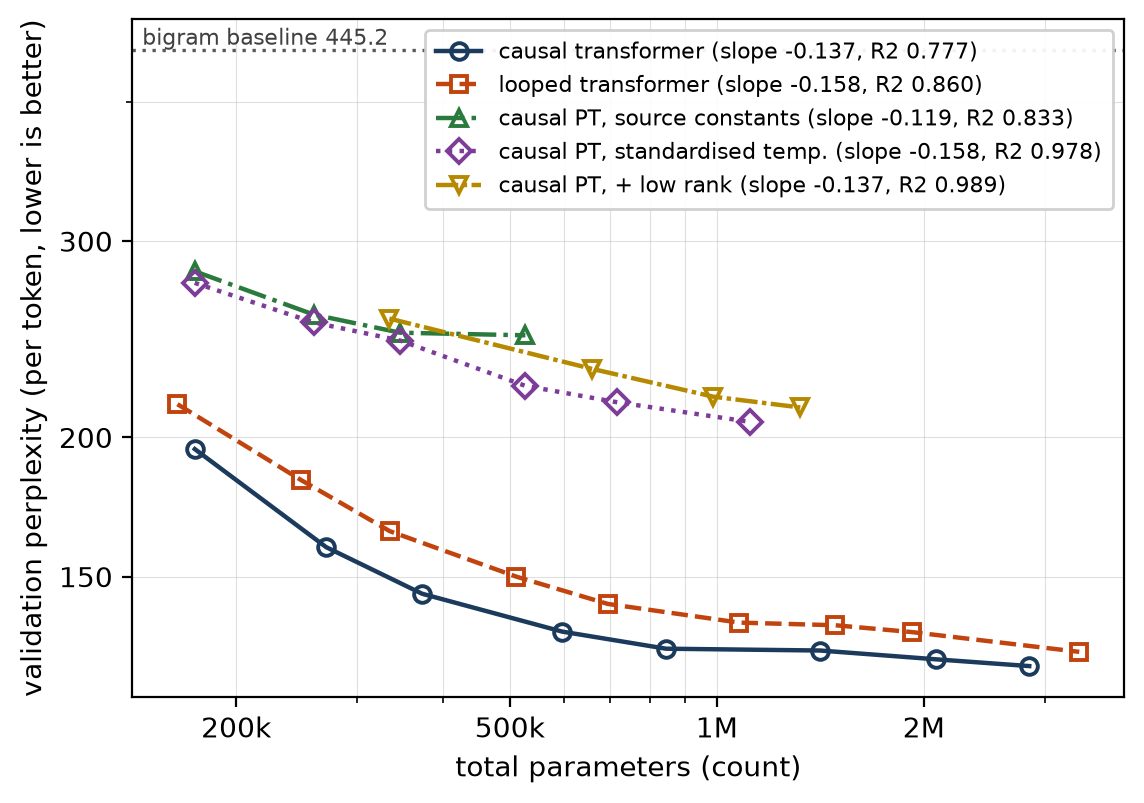
\includegraphics[width=0.85\columnwidth]{figures/fig_scaling_total.png}
\caption{As \Cref{fig:scaling}, against total parameters. With tied embeddings almost all of the
causal PT's parameters are in $\Sfac$.}
\label{fig:scaling-total}
\end{figure}

\begin{table}[t]
\centering\footnotesize
% Generated by `python -m experiments.make_report`. Do not edit by hand.
\begin{tabular}{@{}lrrr@{}}
\toprule
 & $n$ & exponent & ppl across the range \\
\midrule
transformer & 4 & $-0.175$ & $189 \to 124$ \\
looped & 3 & $-0.068$ & $157 \to 133$ \\
PT low rank & 8 & $-0.045$ & $226 \to 203$ \\
\bottomrule
\end{tabular}

\caption{Scaling exponents fitted on the one range all three curves share, \ExpTriLo--\ExpTriHi{}
non-embedding parameters; $n$ is the number of frontier points per fit.}
\label{tab:exponents-trio}
\end{table}

\begin{table*}[t]
\centering\footnotesize
% Generated by `python -m experiments.make_report`. Do not edit by hand.
\begin{tabular}{@{}llrrlrrl@{}}
\toprule
pair & range & $n$ & exponent & leave-one-out & $n$ & exponent & leave-one-out \\
\midrule
transformer / looped & 13k--790k & 6 & $-0.115$ & $-0.148$ to $-0.078$ & 6 & $-0.042$ & $-0.045$ to $-0.034$ \\
looped / causal PT & 4.1k--66k & 4 & $-0.130$ & $-0.145$ to $-0.110$ & 5 & $-0.090$ & $-0.093$ to $-0.090$ \\
looped / PT low rank & 4.2k--148k & 5 & $-0.107$ & $-0.130$ to $-0.088$ & 10 & $-0.058$ & $-0.062$ to $-0.046$ \\
transformer / causal PT & 13k--66k & 3 & $-0.223$ & $n$ too small & 3 & $-0.084$ & $n$ too small \\
transformer / PT low rank & 13k--148k & 4 & $-0.175$ & $-0.223$ to $-0.126$ & 8 & $-0.045$ & $-0.049$ to $-0.042$ \\
\bottomrule
\end{tabular}

\caption{Pairwise exponents, each pair fitted on the range both curves share: number of frontier
points, exponent, and its range when any one point is left out. Where the two leave-one-out
ranges in a row do not overlap, no single point decides the ordering. Two rows rest on three
points a side, the minimum for a fit and too few to leave one out.}
\label{tab:exponents-full}
\end{table*}

\subsection{Width, temperature and rank}
\label{app:grid-gain}
\label{app:grid-lr}
\label{app:grid-rank}

\paragraph{Width.}
Undamped at the original temperature, $\nlab=32$, $96$ and $128$ end at $700.7$, $698.1$ and
$701.4$ (\Cref{fig:width-alpha}). The best damping step is at the edge of the grid at five of
seven widths, and we did not sweep below $\alpha_Z=0.125$. With the damped constants tuned at
$\nlab=32$, the model becomes unpredictable at larger widths, not gradually worse: $253.0\pm6.0$
at $\nlab=32$, $287.4\pm52.5$ at $48$ and $470.0\pm160.7$ at $64$. The growing standard
deviation matters more than the mean. Under the standardised temperature, undamped, the full
ladder reaches $229.8\pm8.5$ at $\nlab=48$ and $219.8\pm4.2$ at $\nlab=64$
(\Cref{tab:fullrank}). \Cref{fig:mechanism} separates two failures that end on the same unigram perplexity: at $\nlab=96$ the beliefs never leave the uniform point, while at $\nlab=32$ they sharpen to $5.5$,
hold for about $2{,}000$ steps and collapse, the feedback loop of \Cref{sec:temperature}.

\paragraph{Gain.}
We swept the gain over $\{1, 1.5, 2, 3, 4, 6\}$ at four widths (\Cref{tab:gain}). The argmin
does not depend on width because, after standardisation, the attention entropy depends on the
gain and the size of the head domain but not on $\nlab$. At $\nlab\ge96$ the working range
shrinks to gain $1$, the width ceiling of \Cref{sec:exp-width}. Above the range the
failure is reproducible: at $\nlab=32$, gain $3$ collapses all three seeds ($700.5\pm0.7$).

\paragraph{Learning rate.}
\Cref{tab:lr} is the diagnostic used for maximal update parameterisation \citep{yang2022tensor},
which \citet{kuang2026scaling} apply to the encoder. Over an eightfold range of width the argmin
moves by one step of the $2\times$ grid in both arms: from $2\times10^{-2}$ to $10^{-2}$ under the
original temperature and from $4\times10^{-2}$ to $2\times10^{-2}$ under the standardised one.
With one seed per cell, the argmin under the original temperature is within seed noise.

\paragraph{Rank.}
The arc scores factor as $\Tfac{c} = \Ufac{c}\Vfac{c}{}^{\!\top}$ with
$\Ufac{c},\Vfac{c}\in\R^{\nlab\times\krank}$. \citet{wu2023probabilistic} set
$\krank=\min(64,\nlab)$ in their Table~2, which for $\nlab\le64$ is $\krank=\nlab$, the most expensive choice. At $\nlab=96$, halving the rank to
$\krank=48$ improves perplexity and cuts the seed spread eightfold (\Cref{tab:rank}); $\krank=12$
gives $257.8\pm4.5$ with eight times fewer non-embedding parameters and still beats the best
$\nlab=32$ configuration of comparable size. The arc score enters inference only as
$\Bfac{c}_{j,a} = \E_{\qbar{j}}[\Tfac{c}_{a,\cdot}]$, so only its rank on the affine hull of the
reachable beliefs is used, and these beliefs are measurably concentrated. On the full ladder, low
rank sits below $\krank=\nlab$ ($223.1\pm5.6$ at $18{,}624$ non-embedding parameters against
$372\pm277$ for $\krank=96$ at $147{,}648$, a mean that includes one collapsed seed). It trains stably through $\nlab=\LadderTopLab$,
$\krank=\LadderTopRank$, with seed standard deviations from $\LadderSdLo$ to $\LadderSdHi$ over
the \LadderNok{} configurations that trained (\Cref{tab:main}), but one seed in three still
collapses at $\nlab=256$, $\krank=64$, the widest and highest-rank cell.

\begin{figure}[t]
\centering
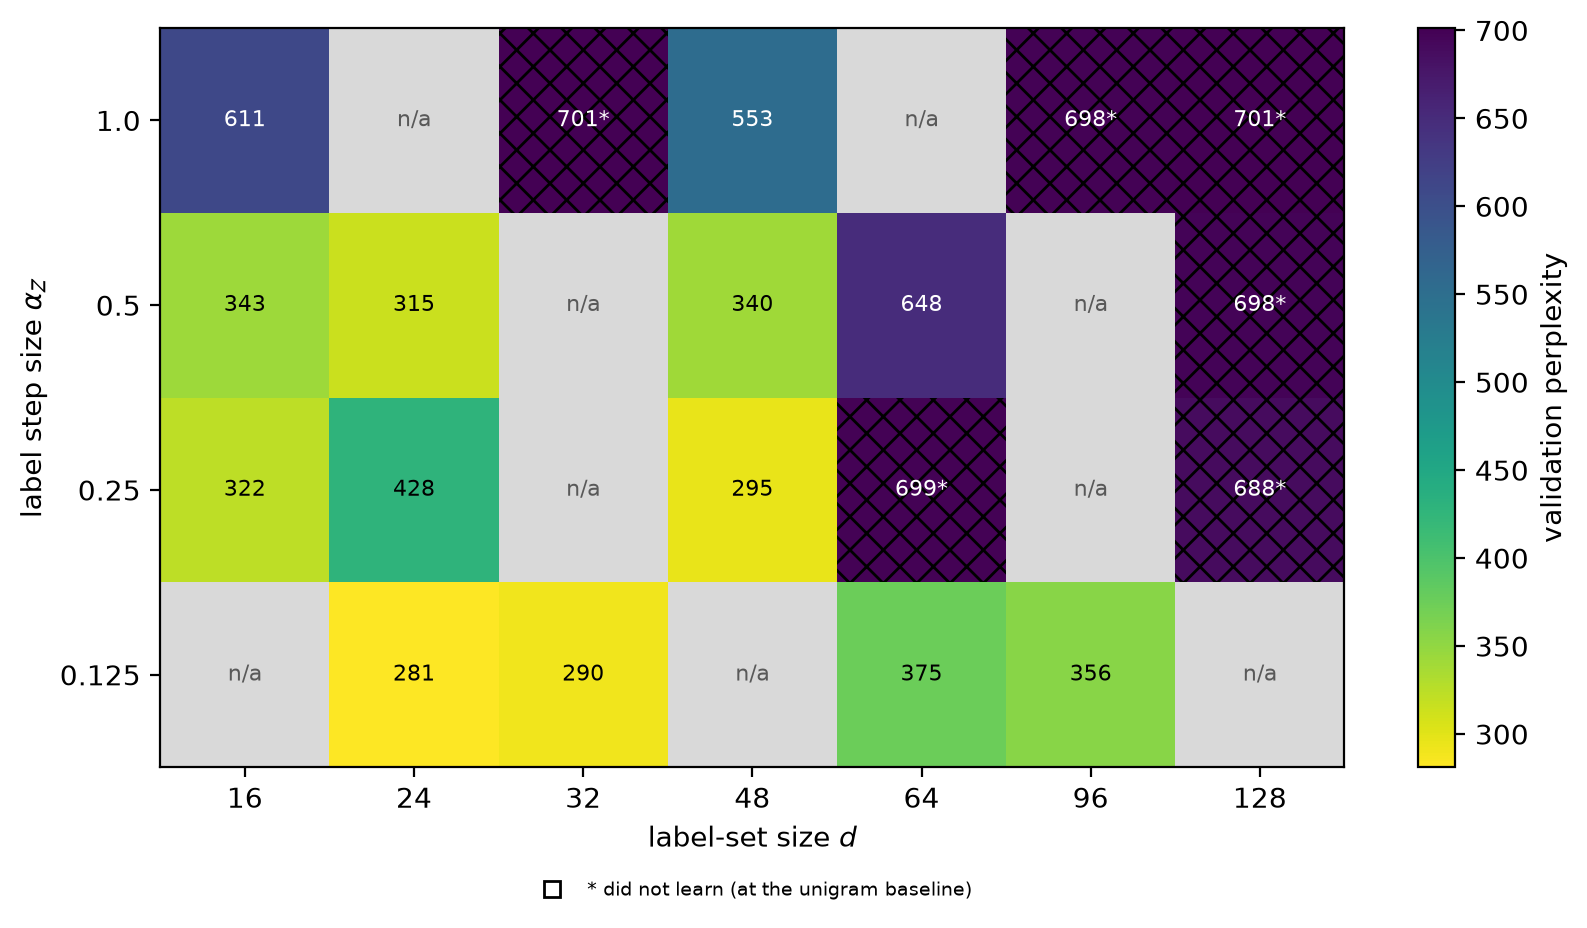
\includegraphics[width=0.85\columnwidth]{figures/fig_width_alpha.png}
\caption{Label-set size against damping step $\alpha_Z$ on PTB at the original temperature
$\lamH=1/\nlab$, $6{,}000$ steps; hatched cells finished on the unigram, grey cells were not
run.}
\label{fig:width-alpha}
\end{figure}

\begin{figure}[t]
\centering
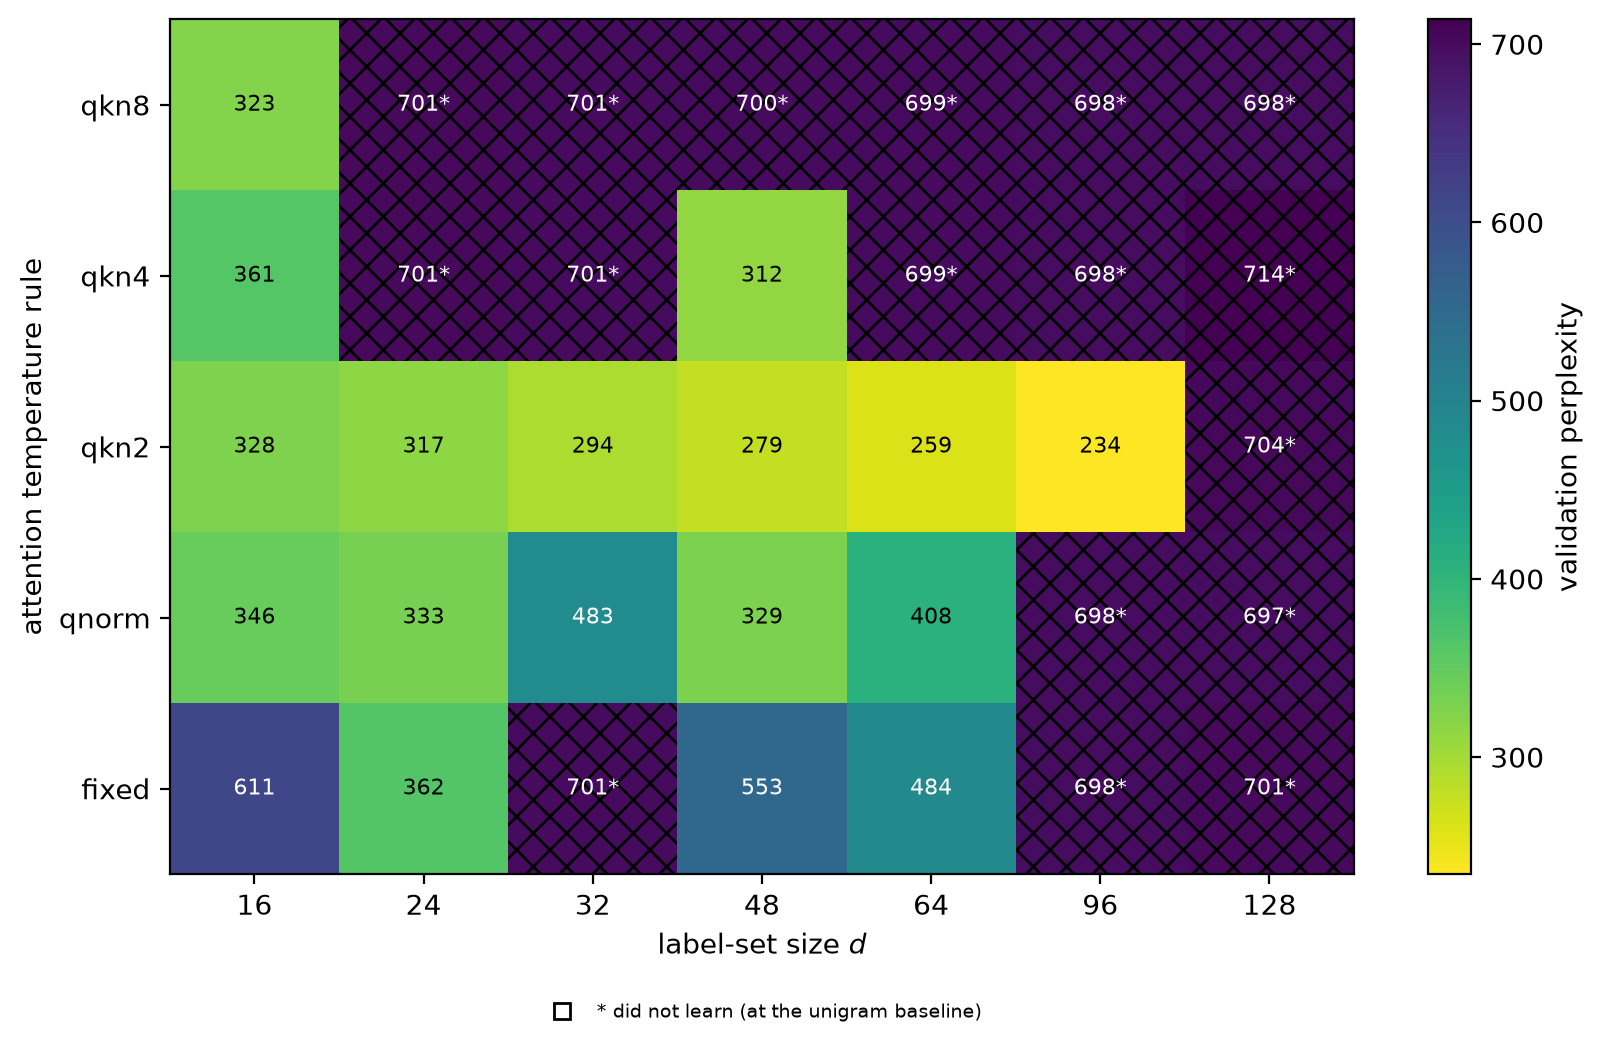
\includegraphics[width=0.85\columnwidth]{figures/fig_width_temp.png}
\caption{Label-set size against the head-temperature rule on PTB, undamped, $6{,}000$ steps.
`fixed' is the
original temperature, `qnorm' the belief-norm temperature and `qkn$g$' the standardised
temperature at gain $g$; hatched cells finished on the unigram.}
\label{fig:width}
\end{figure}

\begin{figure}[t]
\centering
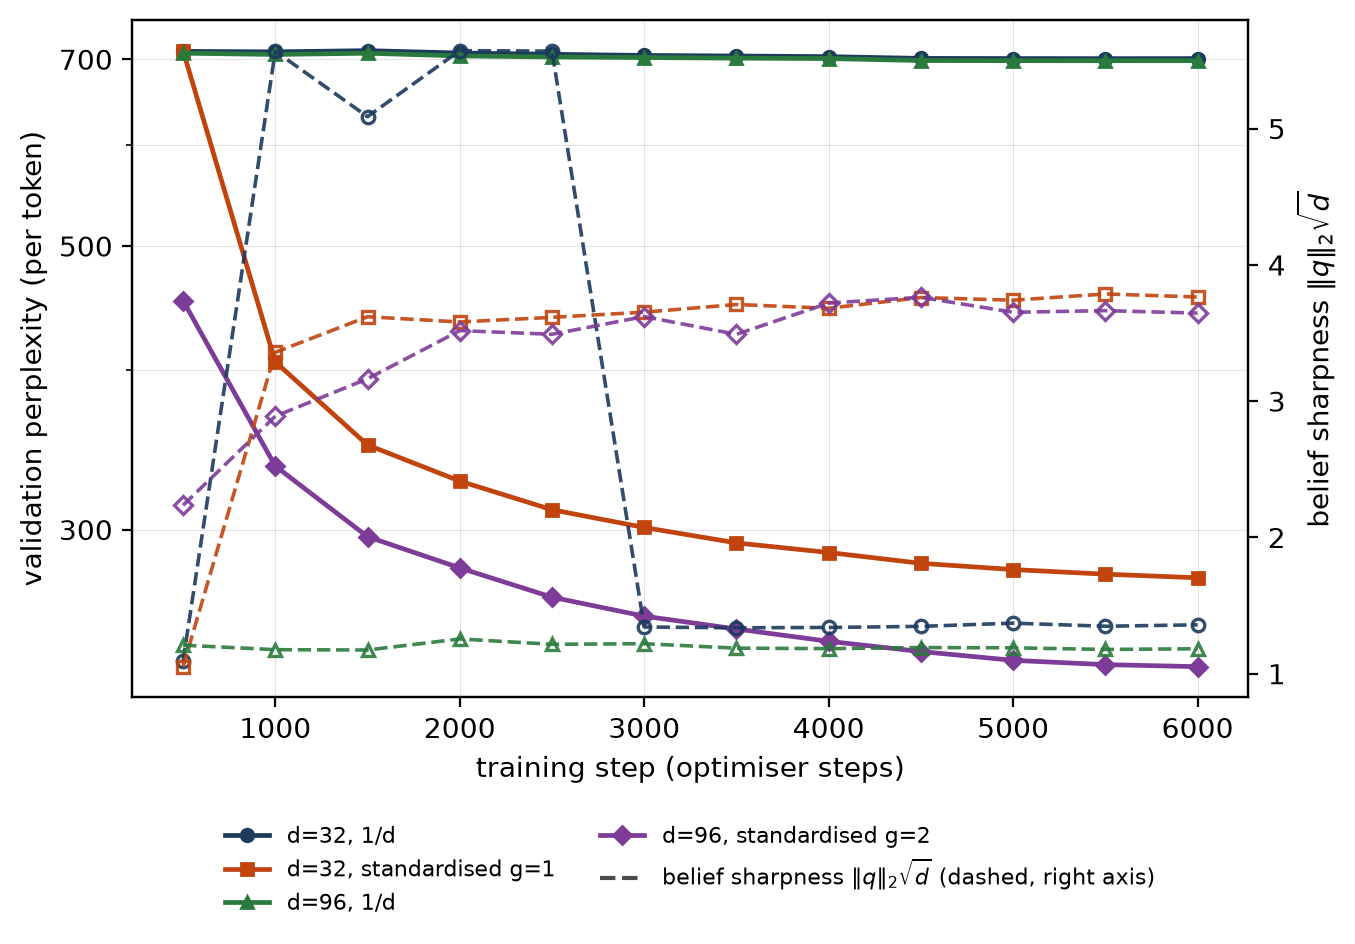
\includegraphics[width=0.85\columnwidth]{figures/fig_mechanism_sharp.png}
\caption{Within-run mechanism, undamped. Solid: validation perplexity (left axis). Dashed: belief
sharpness $\|\QZ{}\|_2\sqrt{\nlab}$ (right axis), $1$ at the uniform belief and $\sqrt{\nlab}$
at a one-hot. At the original temperature the $\nlab=96$ run never leaves the uniform point and
the $\nlab=32$ run sharpens to $5.5$, holds, then collapses. Under the standardised temperature
sharpness rises to a moderate value and stays, and perplexity falls throughout.}
\label{fig:mechanism}
\end{figure}

\begin{table*}[t]
\centering\scriptsize
% Generated by `python -m experiments.make_report`. Do not edit by hand.
\begin{tabular}{llrrrr}
\toprule
Model & Config & Emb. & Non-emb. & Val ppl & Test ppl \\
\midrule
Unigram & --- & --- & --- & 688.8 & --- \\
Causal PT & $d=16$ & 170{,}000 & 4{,}128 & 281.1 $\pm$ 8.5 & 257.2 $\pm$ 7.1 \\
\quad Transformer & $d_{\mathrm{model}}=16$ & 161{,}024 & 13{,}152 & 195.2 & 181.0 \\
\quad Looped & $d_{\mathrm{model}}=16$ & 161{,}024 & 3{,}312 & 214.2 & 196.5 \\
\quad Looped & $d_{\mathrm{model}}=24$ & 241{,}536 & 7{,}272 & 183.1 & 168.4 \\
Causal PT & $d=24$ & 250{,}000 & 9{,}264 & 262.5 $\pm$ 13.6 & 240.4 $\pm$ 12.6 \\
\quad Transformer & $d_{\mathrm{model}}=16$ & 161{,}024 & 13{,}152 & 195.2 & 181.0 \\
\quad Transformer & $d_{\mathrm{model}}=24$ & 241{,}536 & 28{,}944 & 159.4 & 147.2 \\
\quad Looped & $d_{\mathrm{model}}=24$ & 241{,}536 & 7{,}272 & 183.1 & 168.4 \\
\quad Looped & $d_{\mathrm{model}}=32$ & 322{,}048 & 12{,}768 & 164.7 & 150.1 \\
Causal PT & $d=32$ & 330{,}000 & 16{,}448 & 246.7 $\pm$ 2.7 & 224.7 $\pm$ 3.5 \\
\quad Transformer & $d_{\mathrm{model}}=24$ & 241{,}536 & 28{,}944 & 159.4 & 147.2 \\
\quad Transformer & $d_{\mathrm{model}}=32$ & 322{,}048 & 50{,}880 & 144.8 & 133.9 \\
\quad Looped & $d_{\mathrm{model}}=32$ & 322{,}048 & 12{,}768 & 164.7 & 150.1 \\
\quad Looped & $d_{\mathrm{model}}=48$ & 483{,}072 & 28{,}368 & 150.0 & 137.2 \\
Causal PT & $d=48$ & 490{,}000 & 36{,}960 & 229.8 $\pm$ 8.5 & 210.3 $\pm$ 7.5 \\
\quad Transformer & $d_{\mathrm{model}}=32$ & 322{,}048 & 50{,}880 & 144.8 & 133.9 \\
\quad Transformer & $d_{\mathrm{model}}=48$ & 483{,}072 & 113{,}184 & 133.9 & 122.3 \\
\quad Looped & $d_{\mathrm{model}}=48$ & 483{,}072 & 28{,}368 & 150.0 & 137.2 \\
\quad Looped & $d_{\mathrm{model}}=64$ & 644{,}096 & 50{,}112 & 141.8 & 129.7 \\
Causal PT & $d=64$ & 650{,}000 & 65{,}664 & 219.8 $\pm$ 4.2 & 201.3 $\pm$ 3.4 \\
\quad Transformer & $d_{\mathrm{model}}=48$ & 483{,}072 & 113{,}184 & 133.9 & 122.3 \\
\quad Transformer & $d_{\mathrm{model}}=64$ & 644{,}096 & 200{,}064 & 129.2 & 118.2 \\
\quad Looped & $d_{\mathrm{model}}=64$ & 644{,}096 & 50{,}112 & 141.8 & 129.7 \\
\quad Looped & $d_{\mathrm{model}}=96$ & 966{,}144 & 112{,}032 & 136.4 & 125.9 \\
Causal PT & $d=96$ & 970{,}000 & 147{,}648 & 372.4 $\pm$ 277.0 & 340.4 $\pm$ 251.2 \\
\quad Transformer & $d_{\mathrm{model}}=64$ & 644{,}096 & 200{,}064 & 129.2 & 118.2 \\
\quad Transformer & $d_{\mathrm{model}}=96$ & 966{,}144 & 447{,}552 & 128.8 & 118.7 \\
\quad Looped & $d_{\mathrm{model}}=96$ & 966{,}144 & 112{,}032 & 136.4 & 125.9 \\
\quad Looped & $d_{\mathrm{model}}=128$ & 1{,}288{,}192 & 198{,}528 & 135.7 & 124.4 \\
Causal PT & $d=128$ & 1{,}290{,}000 & 262{,}400 & 508.9 $\pm$ 186.9 & 465.6 $\pm$ 171.6 \\
\quad Transformer & $d_{\mathrm{model}}=96$ & 966{,}144 & 447{,}552 & 128.8 & 118.7 \\
\quad Transformer & $d_{\mathrm{model}}=128$ & 1{,}288{,}192 & 793{,}344 & 126.5 & 118.1 \\
\quad Looped & $d_{\mathrm{model}}=128$ & 1{,}288{,}192 & 198{,}528 & 135.7 & 124.4 \\
\quad Looped & $d_{\mathrm{model}}=160$ & 1{,}610{,}240 & 309{,}600 & 133.8 & 125.3 \\
\bottomrule
\end{tabular}

\caption{The full-rank ladder ($\krank=\nlab$) under the standardised temperature, each causal
PT row (three seeds) followed by the nearest measured baselines (better of two learning rates).
Embedding and non-embedding parameters are listed separately. Unlike the other tables, rows here
average collapsed seeds in.}
\label{tab:fullrank}
\end{table*}

\begin{table}[t]
\centering\scriptsize
% Generated by `python -m experiments.make_report`. Do not edit by hand.
\begin{tabular}{rrrlr}
\toprule
$d$ & gain & $n$ & val ppl & collapsed \\
\midrule
32 & 1.0 & 3 & 282.2 $\pm$ 6.6 & 0 \\
32 & 1.5 & 3 & 302.7 $\pm$ 26.6 & 0 \\
32 & 2.0 & 3 & 290.5 $\pm$ 8.4 & 0 \\
32 & 3.0 & 3 & 700.5 $\pm$ 0.7 & 3 \\
32 & 4.0 & 3 & 570.9 $\pm$ 225.1 & 2 \\
32 & 6.0 & 3 & 616.0 $\pm$ 147.1 & 2 \\
64 & 1.0 & 3 & 254.0 $\pm$ 1.9 & 0 \\
64 & 1.5 & 3 & 262.3 $\pm$ 3.6 & 0 \\
64 & 2.0 & 3 & 260.3 $\pm$ 0.8 & 0 \\
64 & 3.0 & 3 & 415.3 $\pm$ 245.2 & 1 \\
64 & 4.0 & 3 & 631.9 $\pm$ 116.0 & 2 \\
64 & 6.0 & 3 & 673.8 $\pm$ 49.0 & 2 \\
96 & 1.0 & 3 & 275.6 $\pm$ 27.1 & 0 \\
96 & 1.5 & 3 & 548.0 $\pm$ 276.0 & 2 \\
96 & 2.0 & 3 & 418.4 $\pm$ 260.6 & 1 \\
96 & 3.0 & 3 & 702.6 $\pm$ 7.4 & 3 \\
96 & 4.0 & 3 & 582.1 $\pm$ 201.3 & 2 \\
96 & 6.0 & 3 & 698.6 $\pm$ 0.5 & 3 \\
128 & 1.0 & 3 & 433.6 $\pm$ 205.6 & 0 \\
128 & 1.5 & 3 & 601.7 $\pm$ 186.4 & 2 \\
128 & 2.0 & 3 & 709.7 $\pm$ 5.9 & 3 \\
128 & 3.0 & 3 & 690.6 $\pm$ 13.1 & 3 \\
128 & 4.0 & 3 & 704.6 $\pm$ 11.1 & 3 \\
128 & 6.0 & 3 & 698.1 $\pm$ 0.4 & 3 \\
\bottomrule
\end{tabular}

\caption{Validation perplexity by label-set size and standardisation gain; three seeds, undamped,
$6{,}000$ steps; `collapsed' counts seeds on the unigram. The argmin is $1$ at every width; the
working range is $[1,2]$ at $\nlab\in\{32,64\}$, and at $\nlab\in\{96,128\}$ only gain $1$ avoids
collapse.}
\label{tab:gain}
\end{table}

\begin{table}[t]
\centering\footnotesize\setlength{\tabcolsep}{3pt}
% Generated by `python -m experiments.make_report`. Do not edit by hand.
\begin{tabular}{rlrrrrrr}
\toprule
$d$ & temperature & 0.005 & 0.01 & 0.02 & 0.04 & 0.08 & argmin \\
\midrule
16 & source & 697 & 641 & 430 & 662 & 708 & 0.02 \\
16 & standardised & 697 & 701 & 334 & 300 & 305 & 0.04 \\
32 & source & 696 & 502 & 674 & 716 & 710 & 0.01 \\
32 & standardised & 696 & 350 & 294 & 288 & 714 & 0.04 \\
64 & source & 696 & 359 & 664 & 700 & 711 & 0.01 \\
64 & standardised & 696 & 658 & 258 & 710 & 714 & 0.02 \\
128 & source & 694 & 499 & 607 & 716 & 709 & 0.01 \\
128 & standardised & 694 & 442 & 416 & 713 & 721 & 0.02 \\
\bottomrule
\end{tabular}

\caption{Validation perplexity against learning rate; one seed, undamped, $6{,}000$ steps.
`source' is the original temperature $\lamH=1/\nlab$, `standardised' the standardised one at
gain $2$. In
both arms the argmin moves by one grid step over an eightfold range of width.}
\label{tab:lr}
\end{table}

\begin{table}[t]
\centering\footnotesize
% Generated by `python -m experiments.make_report`. Do not edit by hand.
\begin{tabular}{rrrrl}
\toprule
$d$ & $r$ & non-emb. & $n$ & val ppl \\
\midrule
32 & 4 & 2{,}112 & 3 & 308.4 $\pm$ 17.2 \\
32 & 8 & 4{,}160 & 3 & 295.8 $\pm$ 1.1 \\
32 & 16 & 8{,}256 & 3 & 294.3 $\pm$ 3.6 \\
32 & 32 & 16{,}448 & 3 & 282.2 $\pm$ 6.6 \\
96 & 12 & 18{,}624 & 3 & 257.8 $\pm$ 4.5 \\
96 & 24 & 37{,}056 & 3 & 256.2 $\pm$ 3.8 \\
96 & 48 & 73{,}920 & 3 & 242.6 $\pm$ 3.3 \\
96 & 96 & 147{,}648 & 3 & 275.6 $\pm$ 27.1 \\
\bottomrule
\end{tabular}

\caption{Validation perplexity against the rank $\krank$ of the arc scores; three seeds,
standardised temperature, undamped, $6{,}000$ steps.}
\label{tab:rank}
\end{table}

\subsection{Global variables and initialisation}
\label{app:grid-globalhead}
\label{app:grid-init}

An initialisation has a treatment (whether $\Bglob$ shares the scale and $L_2$ coefficient of the
other factors) and a draw distribution (Gaussian unless stated). A symmetry can stall the global
variable. If the rows of $\Bglob$ are close relative to their length, the variable's posterior is
uniform, the message is the row mean, and every row gets the same gradient $1/m$, so nothing
separates them, and a shared $L_2$ penalty shrinks whatever spread could.

\paragraph{Original temperature.}
At $\nlab=32$ the model without a global variable collapses ($700.7$), while several
configurations with one reach $323$ to $380$ ($6{,}000$ steps), as if the extra message into
$\Zv{t}$ broke the feedback loop. With one seed per cell (\Cref{tab:init}), Gaussian, uniform and semi-orthogonal draws give
$700.7$, $375.0$ and $386.3$ at $\nlab=32$. Against a seed standard deviation of
$\ReproUndampedSd$ we draw no conclusion from this grid.

\paragraph{Standardised temperature.}
With three seeds, undamped (\Cref{tab:globalhead}), the global variable has no effect at
$\nlab=32$: $243.2\pm5.3$ without it, $242.5$ to $254.1$ with it across three scales and both
$L_2$ treatments; the collapse it rescued at the original temperature is gone. At $\nlab=64$, the edge of the stable region, the model without it is unstable: one seed in
three collapses ($216.8$, $215.1$ and $704.1$). With it, four of six treatments train on every seed
($221$ to $234$). The two that do not are the smallest initialisation outside the shared $L_2$
($224.0$, $616.5$, $639.1$) and the middle one inside it ($215.0$, $235.2$, $667.0$). The largest,
$0.5$, is stable under both treatments; this is the one regularity here, and the opposite of what
the symmetry account predicts. The
global variable changes which configurations are stable; it does not make the model stable.
Otherwise, Gaussian scales spanning $25\times$, with or without the shared $L_2$, change little
else.

\paragraph{Entropy and capacity.}
The entropy $H(Q_g)$ of the global variable's posterior is at least $0.93$ of its maximum in every
cell, even where the variable's message is $1.19$ to $1.52$ times the word unary (outside the shared $L_2$). The
variable thus sends a near-constant label prior, not the feed-forward-like operator it was
proposed as, and perplexity alone cannot show this. Capacity agrees: $m=16$, $64$ and $256$ give
$224.2\pm5.1$, $222.2\pm4.8$ and $222.8\pm4.7$, so sixteen times more values are worth less than
one seed standard deviation.

\paragraph{Draw.}
At $\nlab=64$ (\Cref{tab:draws}), the semi-orthogonal draw's worst seed beats the Gaussian mean,
and the uniform draw collapses on one seed in three. For a model whose main practical problem is
seed variance, this matters more than the difference in means. The symmetry account suggests
that a shared $L_2$ should stall a small Gaussian draw and spare an orthogonal one. Instead the
small Gaussian draw fails outside the shared $L_2$, and the orthogonal draw's advantage is its low
variance. Maximal update parameterisation \citep{yang2022tensor} assumes a Gaussian draw, so its
transfer results may not be neutral to this choice.

\begin{table}[t]
\centering\footnotesize
% Generated by `python -m experiments.make_report`. Do not edit by hand.
\begin{tabular}{@{}rllrr@{}}
\toprule
$\nlab$ & draw & head & val ppl & test ppl \\
\midrule
16 & normal & no & 430.0 & 393.1 \\
16 & orthogonal & no & 346.1 & 314.0 \\
16 & uniform & no & 424.4 & 386.3 \\
32 & normal & no & 700.7 & 641.9 \\
32 & orthogonal & no & 386.3 & 352.3 \\
32 & uniform & no & 375.0 & 341.4 \\
32 & normal & yes & 465.0 & 425.1 \\
32 & orthogonal & yes & 344.9 & 310.0 \\
32 & uniform & yes & 508.8 & 454.2 \\
\bottomrule
\end{tabular}

\caption{Initialisation draw at the original temperature, undamped, one seed per cell,
$6{,}000$ steps. The seed
sd of this configuration is \ReproUndampedSd{} (\Cref{sec:exp-repro}) and the largest difference
here is $326$, so no conclusion is drawn; \Cref{tab:globalhead} repeats the question at three
seeds.}
\label{tab:init}
\end{table}

\begin{table}[t]
\centering\footnotesize
\begin{tabular}{@{}l@{\ \ }l@{\ \ }l@{}}
\toprule
draw & val ppl & seeds \\
\midrule
semi-orthogonal & $219.3 \pm 0.6$ & $218.8$, $219.1$, $219.9$ \\
Gaussian & $225.8 \pm 10.2$ & $214.1$, $229.9$, $233.3$ \\
uniform & \textit{1/3 collapsed} & $225.2$, $272.9$, $707.1$ \\
\bottomrule
\end{tabular}
\caption{Initialisation draw of $\Bglob$ at $\nlab=64$, $m=64$, scale $0.02$, shared $L_2$;
three seeds, with each seed's value.}
\label{tab:draws}
\end{table}

\begin{table*}[t]
\centering\scriptsize
% Generated by `python -m experiments.make_report`. Do not edit by hand.
\begin{tabular}{rrllrrlr}
\toprule
$d$ & $m$ & init sd & in $L_2$ & dist. & $n$ & val ppl & $H(Q_g)/\max$ \\
\midrule
32 & 0 & --- & yes & normal & 3 & 243.2 $\pm$ 5.3 & 0.000 \\
32 & 64 & 0.02 & no & normal & 3 & 249.3 $\pm$ 1.9 & 0.992 \\
32 & 64 & 0.02 & yes & normal & 3 & 242.5 $\pm$ 5.4 & 1.000 \\
32 & 64 & 0.1 & no & normal & 3 & 254.1 $\pm$ 4.4 & 0.976 \\
32 & 64 & 0.1 & yes & normal & 3 & 246.6 $\pm$ 9.8 & 1.000 \\
32 & 64 & 0.5 & no & normal & 3 & 248.4 $\pm$ 3.5 & 0.942 \\
32 & 64 & 0.5 & yes & normal & 3 & 250.3 $\pm$ 9.9 & 0.973 \\
64 & 0 & --- & yes & normal & 3 & \textit{1/3 collapsed} & 0.000 \\
64 & 16 & 0.1 & no & normal & 3 & 224.2 $\pm$ 5.1 & 0.977 \\
64 & 64 & 0.02 & no & normal & 3 & \textit{224--639} & 0.993 \\
64 & 64 & 0.02 & yes & normal & 3 & 225.8 $\pm$ 10.2 & 1.000 \\
64 & 64 & 0.02 & yes & orthogonal & 3 & 219.3 $\pm$ 0.6 & 1.000 \\
64 & 64 & 0.02 & yes & uniform & 3 & \textit{1/3 collapsed} & 1.000 \\
64 & 64 & 0.1 & no & normal & 3 & 222.2 $\pm$ 4.8 & 0.974 \\
64 & 64 & 0.1 & yes & normal & 3 & \textit{215--667} & 1.000 \\
64 & 64 & 0.5 & no & normal & 3 & 221.4 $\pm$ 5.4 & 0.929 \\
64 & 64 & 0.5 & yes & normal & 3 & 228.0 $\pm$ 11.6 & 1.000 \\
64 & 256 & 0.1 & no & normal & 2 & 224.4 $\pm$ 5.3 & 0.988 \\
\bottomrule
\end{tabular}

\caption{The global variable in the standardised configuration of \Cref{sec:exp-width}: number of
values $m$, initialisation sd, whether $\Bglob$ shares the $L_2$ of the other factors, draw,
three seeds. $H(Q_g)/\max$ is the entropy of the global variable's posterior relative to its
maximum; $1.000$ means uniform.}
\label{tab:globalhead}
\end{table*}

\subsection{Switch ladder}
\label{app:grid-switches}

\paragraph{S1.}
Value tying, which the factor graph forces because both roles are the same message through the
same arc factor, costs $-0.6$. Layer normalisation costs $-0.7$ once each switch is tuned; the
$18.5$ it seemed to cost at a single learning rate came from the rate. With the posterior readout
of \Cref{sec:output}, at matched width and with tied embeddings, a transformer does not train: it
ends at $686.8$ (training perplexity $736.6$), and no rate from $10^{-3}$ to $10^{-2}$ does
better. The evaluation swap of
\Cref{sec:exp3} shows weights trained for one readout failing under the other; here a readout
moved into a model built for the other cannot be trained. Together the two show that the mixture
readout is not a drop-in replacement for a linear head. This switch keeps a free projection into
label space (see Caveats), so it is not the causal PT's exact readout.

The simplex state's $+564.3$ is not the cost of the simplex alone. A transformer whose state is
softmaxed after every block has a state norm in $[\nlab^{-1/2}, 1]$ while its attention still
divides by $\sqrt{d_{\text{head}}}$, the miscalibration of \Cref{sec:temperature} seen from the
transformer side. The ladder has no temperature switch, so this interaction lands on the state.
The causal PT, with a simplex state and a temperature suited to it, reaches $\LadderTopVal$. In
\Cref{fig:ladder} the interaction shows as a spike that the readout flip partly undoes.

\paragraph{S2.}
Restoring nine of the ten transformer properties makes the all-PT model worse, by between
$21.5$ (weight sharing) and $392.8$ perplexity (an unconstrained state, which ends on the
unigram). Value tying is the one
neutral change ($+0.7$). The parts of the causal PT therefore depend on each other, which S1
cannot show: there, six of the same properties are free or nearly so.

\paragraph{Caveats.}
The ladder has one seed per cell ($128$ cells), so we draw conclusions only from effects larger
than the seed spread measured in the same regime. The all-PT anchor is best at the top of its
learning-rate grid: four rates gave $687.2$, $395.5$, $354.5$ and $296.7$, and a fifth,
$10^{-1}$, gave $277.3$. The improvements ($-292$, $-41$, $-58$, $-19$) have not turned over, and four of the ten S2 switches also sit at the new boundary. The S2 magnitudes are therefore
lower bounds, though their signs are not in doubt. Every S1 optimum is interior, so the
per-switch attributions rest on S1.

The all-PT model approximates the causal PT in four respects: its mixture readout keeps a free
projection into label space where the causal PT reads the label posterior directly; relative
positions enter as a scalar bias per head and distance bucket, not as a full arc-score matrix
per bucket; heads are concatenated, not summed over channels; and there is no switch for the
damping step or the head temperature. The ladder runs at $\dmodel=\nlab=64$ with four layers
(iterations) and four heads (channels).

\begin{table}[t]
\centering\footnotesize
% Generated by `python -m experiments.make_report`. Do not edit by hand.
\begin{tabular}{lrrrr}
\toprule
switch & S1 val & $\Delta$ & S2 val & $\Delta$ \\
\midrule
attn\_out\_proj & --- & --- & 686.9 & +0.2 \\
attn\_query\_proj & 131.1 & +1.9 & --- & --- \\
attn\_value & 128.7 & -0.6 & --- & --- \\
ffn & 144.4 & +15.1 & 686.9 & +0.3 \\
norm & 128.6 & -0.7 & 686.8 & +0.4 \\
position & 128.9 & -0.4 & --- & --- \\
residual & 136.7 & +7.5 & --- & --- \\
state & 693.8 & +564.5 & --- & --- \\
weight\_sharing & 144.2 & +14.9 & 687.2 & +0.0 \\
\bottomrule
\end{tabular}

\caption{Cost of each difference, measured in two directions. S1: the transformer with that one property replaced by the
causal PT's. S2: the all-PT model with that one property restored to the transformer's. $\Delta$
is measured from the anchor of its own family (the tuned transformer for S1; the all-PT model,
$277.3$, for S2) and signed so that a positive value means the causal PT's version is worse. Best
of four learning rates per switch, one seed per cell. Switch names follow
\Cref{sec:full-comparison}.}
\label{tab:switches}
\end{table}

\begin{figure}[t]
\centering
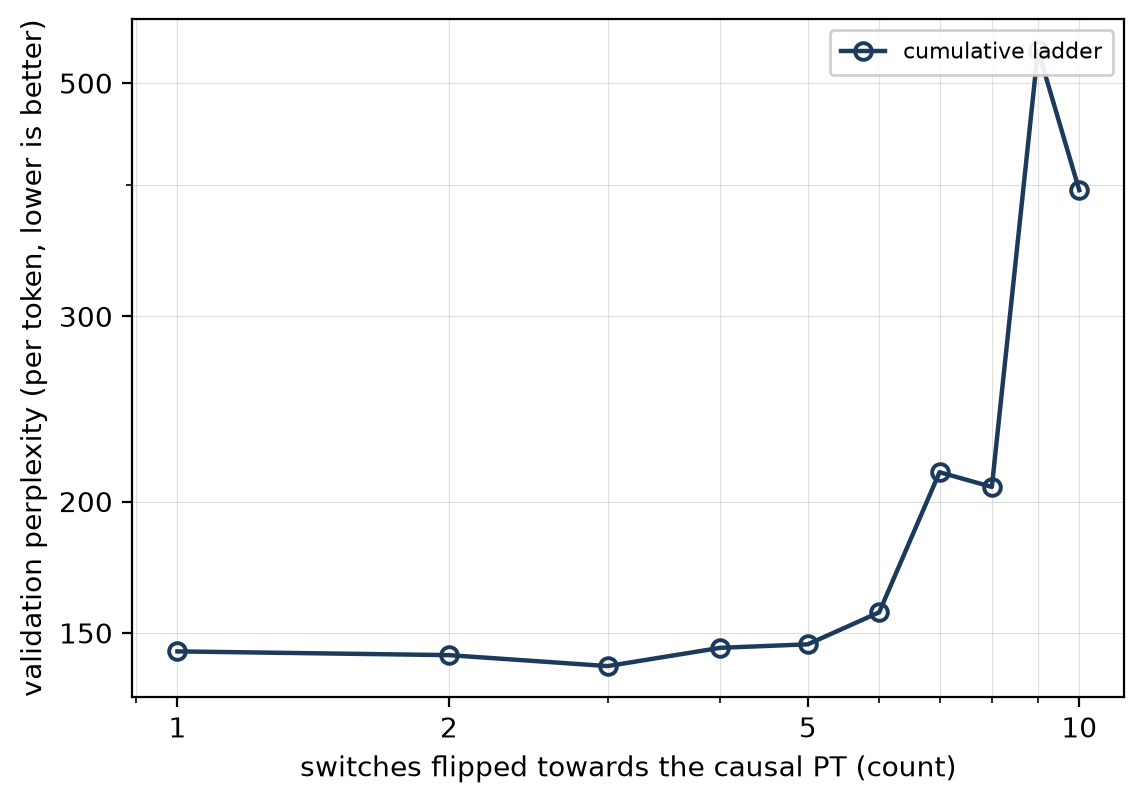
\includegraphics[width=0.85\columnwidth]{figures/fig_switch_ladder.png}
\caption{Cumulative switch ladder: each step flips one more difference from the causal
transformer towards the causal PT and keeps the earlier ones. Each point is the best of the
learning rates run for that step; dotted lines are the tuned endpoints. The last step is the
all-PT model itself. Values in \Cref{tab:switches}.}
\label{fig:ladder}
\end{figure}

\subsection{Constants and inference depth}
\label{app:res-knobs}

All three sweeps use one seed per cell.

\paragraph{$L_2$ on the arc scores.}
Coefficients of $0$, $5\times10^{-5}$, $5\times10^{-4}$, $5\times10^{-3}$ and $5\times10^{-2}$
give $273.3$, $255.6$, $248.3$, $249.8$ and $697.0$. At $5\times10^{-2}$ the arc message is
$2\,\%$ of the word unary and removing the prefix changes the prediction by a KL below
$10^{-8}$: the arc factors have been regularised away. Wu and Tu's value is at or near the
optimum.

\paragraph{Relative-position clip.}
$\clip=1$ and $\clip=3$ give $249.7$ and $248.3$; $\clip=0$ and $\clip=7$ give $619.4$ and
$605.1$, and fail in opposite ways. At $\clip=0$ the model cannot see distance, and the KL from
removing the prefix falls to $0.037$. At $\clip=7$ the arc message reaches eight times the word
unary and the feedback loop of \Cref{sec:temperature} runs away.

\paragraph{Depth.}
Wu and Tu fix $\niter=3$. In the damped configuration at $\nlab=32$ (seed standard deviation
$\ReproDampedSd$), $\niter=1,2,3,5,8$ give $241.3$, $246.5$, $248.3$, $297.0$ and $275.3$, and
$\rho=1,2,4$ predictive rounds (\Cref{app:full-updates}) give $242.1$, $248.3$ and $284.9$; the
middle value is the shared base run ($\niter=3$, $\rho=2$). One seed cannot tell whether the
lower value at $\niter=8$ than at $\niter=5$ is real. The extra iterations may be harmful, since
each re-injects the same arc factors and \Cref{sec:exp-width} shows the feedback loop running
away, or they may only make optimisation harder. Either way, these results do not show whether
computation shared across depth helps at larger scale.

\subsection{Readouts}
\label{app:res-readout}

\begin{table}[t]
\centering\scriptsize\setlength{\tabcolsep}{2pt}
% Generated by `python -m experiments.make_report`. Do not edit by hand.
\begin{tabular}{llrrll}
\toprule
arm & config & non-emb. & $n$ & val ppl & test ppl \\
\midrule
fixed & $d=32$ & 16{,}448 & 3 & 343.1 $\pm$ 24.7 & 321.5 $\pm$ 22.0 \\
fixed & $d=64$ & 65{,}664 & 3 & 334.1 $\pm$ 27.6 & 312.8 $\pm$ 25.7 \\
gpt & $d_{\mathrm{model}}=32$ & 50{,}880 & 2 & 179.7 $\pm$ 4.3 & 167.9 $\pm$ 2.9 \\
gpt & $d_{\mathrm{model}}=64$ & 200{,}064 & 1 & 149.7 $\pm$ 0.0 & 140.8 $\pm$ 0.0 \\
gpt & $d_{\mathrm{model}}=128$ & 793{,}344 & 1 & 144.6 $\pm$ 0.0 & 137.6 $\pm$ 0.0 \\
looped & $d_{\mathrm{model}}=64$ & 50{,}112 & 1 & 168.5 $\pm$ 0.0 & 159.8 $\pm$ 0.0 \\
rule & $d=32$ & 16{,}448 & 3 & 308.1 $\pm$ 2.6 & 288.6 $\pm$ 2.2 \\
rule & $d=64$ & 65{,}664 & 2 & 281.2 $\pm$ 11.7 & 262.6 $\pm$ 11.6 \\
\bottomrule
\end{tabular}

\caption{WikiText-2 with every hyperparameter carried over from PTB. `fixed' and `rule': the
causal PT under the original temperature (damped) and the standardised temperature (undamped),
three seeds; `gpt' and `looped':
causal and looped transformer (two seeds). Unigram $964.8$, bigram $692.5$.}
\label{tab:wt2}
\end{table}

Swapping the readout at evaluation isolates the approximation error; training under each readout
measures the end-to-end effect. The swap is meaningful only at $\lamW=1$
(\Cref{app:message-weights}). Over the \SwapNconfigs{} configurations with three uncollapsed
seeds, the swap takes seed-mean perplexity from $\SwapMildestTrained$ to $\SwapMildestSwapped$ at
the mildest ($\nlab=\SwapMildestLab$, $\krank=\SwapMildestRank$) and from $\SwapWorstTrained$ to
$\SwapWorstSwapped$ at the worst ($\nlab=\SwapWorstLab$, $\krank=\SwapWorstRank$). The exact
logits are not degenerate: they discriminate less between words at a fixed context (standard
deviation $1.63$ against $2.64$ for the mean-field readout) and more between contexts for a fixed
word ($2.73$ against $2.42$). Trained under each readout (one seed each), the exact one is worse
by factors of $1.41$ ($\nlab=32$) and $1.30$ ($\nlab=16$). \Cref{app:worked-example} compares the two readouts
on one slot.

\subsection{Factored labels}
\label{app:grid-factored}

At $\nlab=8$ the affine dimension of the log-conditionals is $8$, $7$ and $5$ for $\ncomp=1,2,4$
under the mean-field readout, never above $\nlab$, and strictly above $\nlab$ under the exact
readout on the same contexts.

\paragraph{Iso-parameter diagonals.}
Factoring shrinks the arc factors but not the word--label factors (\Cref{app:factored}), so we
compare $(\nlab,\ncomp)$ pairs with equal arc budgets (\Cref{tab:factored}). With the mean-field
readout, $8{,}256$ arc parameters give $283.8\pm8.3$ at $(16,1)$, $230.6\pm4.4$ at $(32,2)$ and
$230.5\pm11.0$ at $(64,4)$. At $32{,}896$ the seeds disagree at $(32,1)$, and $(64,2)$ gives
$220.6\pm3.2$. The extra label width that factoring allows is worth about $50$ perplexity, most
of it in the first halving.

\paragraph{Readout penalty.}
The exact readout's penalty falls monotonically with $\ncomp$ on both diagonals
(\Cref{tab:penalty}). At $\ncomp=1$ the product of $\ncomp$ mixtures is one mixture, so the
richer family has nothing extra to express; splitting the label variable gives it something. At
$\ncomp=4$ the exact readout is also the stable one ($\pm0.8$ and $\pm4.6$ against $\pm11.0$ and
$\pm9.4$). The sign change at $\ncomp=4$ ($-3.5$ and $-6.2$) is within a seed spread, so we claim
only the downward trend across the five measured cells on two budgets.

\paragraph{Fixed width.}
At $\nlab=32$, raising $\ncomp$ cuts the arc budget to $32{,}896$, $8{,}256$ and $2{,}080$. The
exact readout improves throughout ($313.0\pm9.5$, $260.6\pm1.4$, $253.0\pm1.7$) as $94\,\%$ of the
arc parameters go. The mean-field readout gives $230.6\pm4.4$ at $\ncomp=2$ and $250.5\pm7.0$ at
$\ncomp=4$, and its seeds disagree at $\ncomp=1$. This is the only setting in which the exact
readout improves as the arc budget shrinks; at $\ncomp=4$ it matches the mean-field readout with
a quarter of its seed spread. At $\nlab=64$, $\ncomp=1$ ($131{,}328$ arc parameters), the mean-field readout
collapses on all seeds while the exact one trains to $460.1\pm14.1$: the two do not fail together.
None of this recommends $\ncomp=4$. The best cell is the mean-field model at $\nlab=32$,
$\ncomp=2$, and every cell is well above the best perplexities in \Cref{tab:main}.

\begin{table}[ht]
\centering\footnotesize
\begin{tabular}{@{}l@{\ \ }r@{\ \ }r@{\ \ }r@{}}
\toprule
arc budget & $\ncomp=1$ & $\ncomp=2$ & $\ncomp=4$ \\
\midrule
$8{,}256$   & $+52.2$ & $+30.0$ & $-3.5$ \\
$32{,}896$  & ---     & $+21.7$ & $-6.2$ \\
\bottomrule
\end{tabular}
\caption{Exact-readout perplexity minus mean-field perplexity at a fixed arc budget, three seeds
per cell. The $\ncomp=1$ cell at $32{,}896$ has seeds that disagree and no mean.}
\label{tab:penalty}
\end{table}

\begin{table}[ht]
\centering\footnotesize
% Generated by `python -m experiments.make_report`. Do not edit by hand.
\begin{tabular}{@{}l@{\ }l@{\ }l@{\ }l@{\ }r@{\ }r@{\ }l@{}}
\toprule
fam. & $\nlab$ & $K$ & readout & $n$ & non-emb. & val ppl \\
\midrule
P & 16 & 1 & exact & 3 & 8{,}256 & 336.0 $\pm$ 6.7 \\
P & 16 & 1 & m.\,field & 3 & 8{,}256 & 283.8 $\pm$ 8.3 \\
P & 32 & 2 & exact & 2 & 8{,}256 & 261.0 $\pm$ 1.6 \\
P & 32 & 2 & m.\,field & 3 & 8{,}256 & 230.6 $\pm$ 4.4 \\
P & 64 & 4 & m.\,field & 3 & 8{,}256 & 230.5 $\pm$ 11.0 \\
P & 32 & 1 & m.\,field & 3 & 32{,}896 & 296.0 $\pm$ 69.0 \\
P & 64 & 2 & m.\,field & 1 & 32{,}896 & 222.0 $\pm$ 0.0 \\
P & 128 & 4 & m.\,field & 1 & 32{,}896 & 213.0 $\pm$ 0.0 \\
\bottomrule
\end{tabular}

\caption{Factored labels, three seeds. Family P walks two iso-parameter diagonals ($8{,}256$ and
$32{,}896$ non-embedding parameters), so $\nlab$ rises with $\ncomp$; family W adds the remaining
fixed-width cells. Family W holds the total width fixed, which is where the prediction of
\Cref{sec:variants} applies; on family P, $\nlab$ rises with $\ncomp$, so a mean-field gain there
comes from label width, not from factoring. Original temperature, $\alpha_Z=0.25$, $\nchan=4$.
Italic ranges
and collapse counts as in the introduction to this appendix.}
\label{tab:factored}
\end{table}

\subsection{WikiText-2}
\label{app:grid-wt2}

Every constant is carried over from PTB, although the vocabulary is about three times larger
(\Cref{tab:wt2}). The standardised temperature's seed spread at $\nlab=32$ is an order of
magnitude tighter than the original temperature's. The gap to the baselines persists: with fewer
non-embedding parameters than the causal PT's $65{,}664$, a causal transformer reaches
$\WtGptNarrow\pm\WtGptNarrowSd$ ($50{,}880$ parameters) and a looped one $167.9\pm0.7$
($50{,}112$), two seeds each. At matched $\dmodel$ the looped transformer loses to the standard
one at every width. At matched non-embedding budget it wins at about $5\times10^4$ parameters
($167.9$ against $179.7$) and loses at about $2\times10^5$ ($157.2$ against $150.9$), the same
size-dependent inversion as on PTB.
